Il est désormais important de voir quelles perspectives offrent la connexion des deux bases données. Ce chapitre explore d'abord les avantages de cette interconnexion pour la recherche, puis présente les méthodes de visualisation qui permettent de clarifier ces connexions.


\section{Bénéfices pour la recherche de la mise en relation des deux bases de données}
La mise en relation des bases de données offre des avantages pour la recherche scientifique.

Pour le projet ThEMA, établir ce lien permettra d'approfondir l'étude déjà bien avancée des sources des \index{Récits exemplaires}récits exemplaires\footnote{Il n'existe pas d'ouvrages offrant une synthèse des sources des récits exemplaires. Les sources diffèrent d'un recueil à l'autre, ce qui rend une telle synthèse irréalisable. Cependant, certaines éditions de sources ainsi que des articles ou chapitres de revues les analysent. La base bibliographique Bibliex, consacrée aux récits exemplaires, mentionne 36 fois le mot « source ». Le liens vers Bibliex : \url{https://www.zotero.org/groups/2304628/bibliex}}. Plus précisément, cela permettra de se concentrer sur les sources encyclopédiques, qui ont jusqu'à présent été peu analysées\footnote{Il n'y a que 6 références aux encyclopédies dans Bibliex}. En examinant ces sources, nous pourrons identifier les thèmes, les sujets, ainsi que les personnages historiques ou bibliques les plus souvent repris de manière globale dans les \textit{exempla} depuis les encyclopédies. Les études des références encyclopédiques dans les recueils de récits exemplaires pourraient dépasser celles déjà réalisées par Marie-Anne Polo de Beaulieu et Jacques Berlioz sur la \textit{Scala Coeli} et le \textit{Tractatus de diversis materiis praedicabilibus}\footcite{berliozRecueilsExemplaDiffusion1994}. Nous pourrons aussi évaluer dans quelle mesure les \index{Récits exemplaires}récits exemplaires d'origine encyclopédique ont été réutilisés par les compilateurs d'\textit{exempla} ultérieurs. Les chercheurs auront l'occasion de comparer la façon dont divers auteurs ou œuvres utilisent les mêmes sources encyclopédiques dans leurs \textit{exempla}, mettant en lumière des variations stylistiques, théologiques ou culturelles. En outre, cette recherche pourrait conduire à la découverte de nouveaux \index{Récits exemplaires}récits exemplaires, étant donné que les \index{Encyclopédies}encyclopédies sont riches en textes inexplorés.

Côté SourcEncyMe, la mise en relation des deux bases pourrait éclairer les raisons pour lesquelles un auteur encyclopédique utilise un \textit{exemplum}\footnote{Il n'existe pas d'étude spécifique sur l'utilisation des récits exemplaires dans les encyclopédies, bien que le lien entre encyclopédies et \textit{exempla} ait déjà été établi, comme je l'ai mentionné dans l'introduction. La bibliographie sur les encyclopédies médiévales réalisée par Isabelle Draelants ne comporte que quelques rares mentions de récits exemplaires. Pour accéder à cette bibliographie, consultez : \url{https://ateliervdb.hypotheses.org/bibliographie-sur-lencyclopedisme-medieval}}. Cela permettra de comprendre pourquoi un auteur intègre un récit habituellement utilisé comme \textit{exemplum} dans son \index{Encyclopédies}encyclopédie, même si celui-ci ne sert pas nécessairement d'exemple. Cette démarche pourrait aussi révéler si des \index{Récits exemplaires}récits exemplaires issus de recueils d'\textit{exempla} sont repris dans des encyclopédies et pour quelles raisons. Elle offrira la possibilité d'analyser plus en profondeur la place des \index{Récits exemplaires}récits exemplaires dans les œuvres encyclopédiques, ainsi que les raisons pour lesquelles ils sont insérés dans certaines sections d'une œuvre et non dans d'autres. 


\section{Techniques de visualisation pour les relations entre \index{Récits exemplaires}récits exemplaires et \index{Encyclopédies}encyclopédies}
Pour continuer la mise en relation des bases de données, plusieurs possibilités de visualisation des données pourraient être envisagées. Elles permettraient aux chercheurs et aux utilisateurs de mieux saisir visuellement les liens entre les encyclopédies et les récits exemplaires. Une pratique de plus en plus en plus utilisée par les chercheurs dans leurs publications\footcite{jiangLiteratureReviewDevelopment2023}. \\

\begin{figure}[H]
	\centering
	\fbox{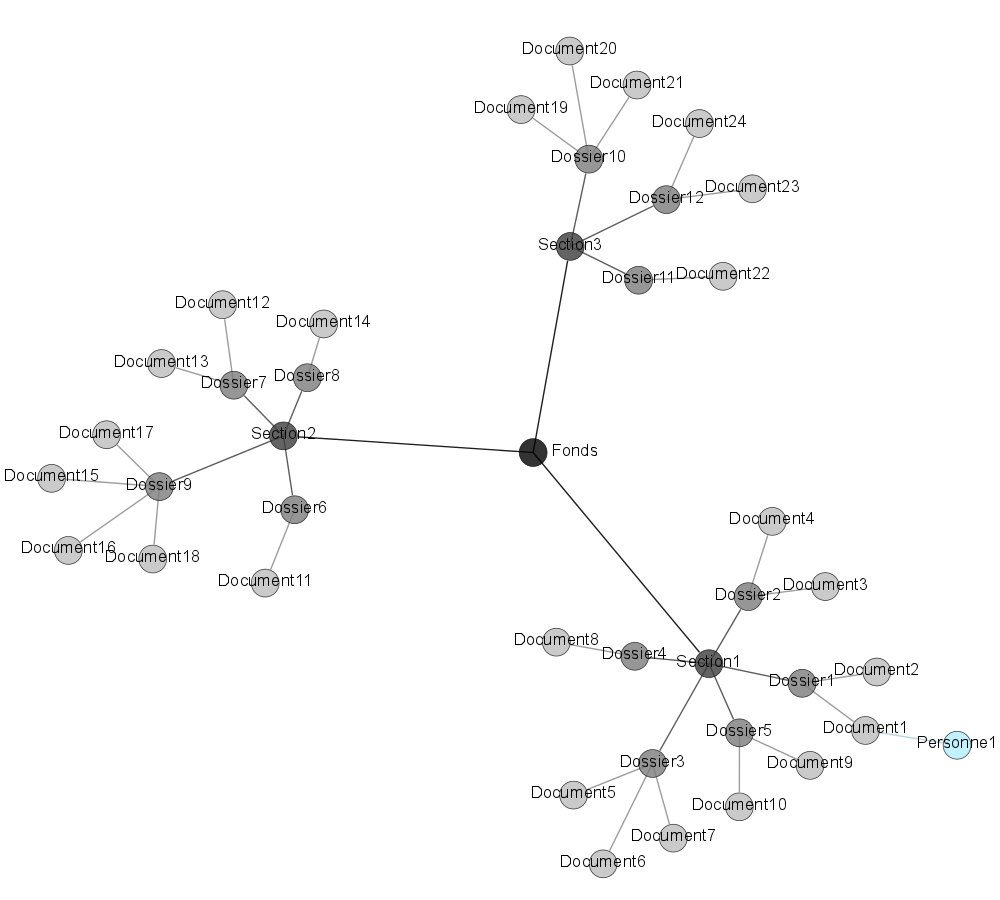
\includegraphics[width=0.2\linewidth]{images/ArchivesExemplePersonne.png}}
	\caption{Exemple de visualisation d'analyse de réseaux}
\end{figure}

Une approche intéressante serait la création de cartographies des liens établis par le travail de mise en relation des deux bases de données comme une sorte d'analyse de réseaux\footcite{beauguitteAnalyseReseauxSciences2016}. Par exemple, si plusieurs recueils d'\textit{exempla} reprennent un même morceau d'encyclopédie ils seront connectés avec des traits vers un unique point matérialisant le texte de l'\index{Encyclopédies}encyclopédie. Ces visualisations de réseaux pourraient permettre de représenter et de mieux saisir les emprunts et les influences entre les deux types de documents. 

Une autre approche intéressante serait celle du graphe de citation c'est à dire une représentation visuelle des relations de citation entre différents éléments, dans ce cas, entre les récits exemplaires au sein des \index{Encyclopédies}encyclopédies et les chapitres des encyclopédies. Le graphe de citations permet de voir rapidement quels \index{Récits exemplaires}récits exemplaires sont cités dans quels chapitres des \index{Encyclopédies}encyclopédies. Chaque lien entre un récit exemplaire et un chapitre montre une relation de citation, c'est-à-dire que le chapitre utilise ou mentionne ce récit. Si un récit exemplaire apparaît dans plusieurs chapitres, il sera connecté à chacun d'eux par des liens distincts. Cela montre non seulement où le récit est utilisé, mais aussi l'étendue de son influence à travers \index{Encyclopédies}l'encyclopédie.

Pour mettre en œuvre ces visualisations, il serait nécessaire d'adapter les fichiers XML selon les TEI Guidelines pour intégrer les métadonnées et annotations nécessaires\footcite{20GraphsNetworks}. Il faudrait ensuite avoir des logiciels comme Gephi\footcite{GephiOpenGraph} ou Cytoscape\footcite{CytoscapeOpenSource} pour développer les représentations. Pour ce qui est de l'analyse de réseaux il faudrait peut être un middleware car les deux bases de données restent séparées. Un middleware est un logiciel qui agit comme une passerelle entre des applications, outils et bases de données. 